% A LaTeX (non-official) template for ISAE projects reports
% Copyright (C) 2014 Damien Roque
% Version: 0.2
% Author: Damien Roque <damien.roque_AT_isae.fr>

\documentclass[a4paper,12pt, openany]{book}
\usepackage[utf8]{inputenc}
\usepackage[T1]{fontenc}
\usepackage[frenchb]{babel} % If you write in French
%\usepackage[english]{babel} % If you write in English
\usepackage{a4wide}
\usepackage{graphicx}
\graphicspath{{images/}} % emplacement des images
\usepackage{subfig}
 \usepackage{float}
\usepackage{tikz}
\usetikzlibrary{shapes,arrows}
\usepackage{pgfplots}
\pgfplotsset{compat=newest}
\pgfplotsset{plot coordinates/math parser=false}
\newlength\figureheight
\newlength\figurewidth
\pgfkeys{/pgf/number format/.cd,
set decimal separator={,\!},
1000 sep={\,},
}
\usepackage{ifthen}
\usepackage{ifpdf}
\ifpdf
\usepackage[pdftex]{hyperref}
\else
\usepackage{hyperref}
\fi
\usepackage{color}
\hypersetup{%
colorlinks=true,
linkcolor=blue,
citecolor=black,
urlcolor=black}

\usepackage{titlesec}
\titleformat{\chapter}[hang]{\bf\huge}{\thechapter}{2pc}{}

\renewcommand{\thesection}{\Roman{section}}


\renewcommand{\baselinestretch}{1.05}
\usepackage{fancyhdr}
\pagestyle{fancy}
\fancyfoot{}
\fancyhead[LE,RO]{\bfseries\thepage}
\fancyhead[RE]{\bfseries\nouppercase{\leftmark}}
\fancyhead[LO]{\bfseries\nouppercase{\rightmark}}
\setlength{\headheight}{15pt}

\let\headruleORIG\headrule
\renewcommand{\headrule}{\color{black} \headruleORIG}
\renewcommand{\headrulewidth}{1.0pt}
\usepackage{colortbl}
\arrayrulecolor{black}

\fancypagestyle{plain}{
  \fancyhead{}
  \fancyfoot[C]{\thepage}
  \renewcommand{\headrulewidth}{0pt}
}

\makeatletter
\def\@textbottom{\vskip \z@ \@plus 1pt}
\let\@texttop\relax
\makeatother

\makeatletter
\def\cleardoublepage{\clearpage\if@twoside \ifodd\c@page\else%
  \hbox{}%
  \thispagestyle{empty}%
  \newpage%
  \if@twocolumn\hbox{}\newpage\fi\fi\fi}
\makeatother

\usepackage{amsthm}
\usepackage{amssymb,amsmath,bbm}
\usepackage{array}
\usepackage{bm}
\usepackage{multirow}
\usepackage[footnote]{acronym}

\newcommand*{\SET}[1]  {\ensuremath{\mathbf{#1}}}
\newcommand*{\VEC}[1]  {\ensuremath{\boldsymbol{#1}}}
\newcommand*{\FAM}[1]  {\ensuremath{\boldsymbol{#1}}}
\newcommand*{\MAT}[1]  {\ensuremath{\boldsymbol{#1}}}
\newcommand*{\OP}[1]  {\ensuremath{\mathrm{#1}}}
\newcommand*{\NORM}[1]  {\ensuremath{\left\|#1\right\|}}
\newcommand*{\DPR}[2]  {\ensuremath{\left \langle #1,#2 \right \rangle}}
\newcommand*{\calbf}[1]  {\ensuremath{\boldsymbol{\mathcal{#1}}}}
\newcommand*{\shift}[1]  {\ensuremath{\boldsymbol{#1}}}

\newcommand{\eqdef}{\stackrel{\mathrm{def}}{=}}
\newcommand{\argmax}{\operatornamewithlimits{argmax}}
\newcommand{\argmin}{\operatornamewithlimits{argmin}}
\newcommand{\ud}{\, \mathrm{d}}
\newcommand{\vect}{\text{Vect}}
\newcommand{\sinc}{\ensuremath{\mathrm{sinc}}}
\newcommand{\esp}{\ensuremath{\mathbb{E}}}
\newcommand{\hilbert}{\ensuremath{\mathcal{H}}}
\newcommand{\fourier}{\ensuremath{\mathcal{F}}}
\newcommand{\sgn}{\text{sgn}}
\newcommand{\intTT}{\int_{-T}^{T}}
\newcommand{\intT}{\int_{-\frac{T}{2}}^{\frac{T}{2}}}
\newcommand{\intinf}{\int_{-\infty}^{+\infty}}
\newcommand{\Sh}{\ensuremath{\boldsymbol{S}}}
\newcommand{\C}{\SET{C}}
\newcommand{\R}{\SET{R}}
\newcommand{\Z}{\SET{Z}}
\newcommand{\N}{\SET{N}}
\newcommand{\K}{\SET{K}}
\newcommand{\reel}{\mathcal{R}}
\newcommand{\imag}{\mathcal{I}}
\newcommand{\cmnr}{c_{m,n}^\reel}
\newcommand{\cmni}{c_{m,n}^\imag}
\newcommand{\cnr}{c_{n}^\reel}
\newcommand{\cni}{c_{n}^\imag}
\newcommand{\tproto}{g}
\newcommand{\rproto}{\check{g}}
\newcommand{\LR}{\mathcal{L}_2(\SET{R})}
\newcommand{\LZ}{\ell_2(\SET{Z})}
\newcommand{\LZI}[1]{\ell_2(\SET{#1})}
\newcommand{\LZZ}{\ell_2(\SET{Z}^2)}
\newcommand{\diag}{\operatorname{diag}}
\newcommand{\noise}{z}
\newcommand{\Noise}{Z}
\newcommand{\filtnoise}{\zeta}
\newcommand{\tp}{g}
\newcommand{\rp}{\check{g}}
\newcommand{\TP}{G}
\newcommand{\RP}{\check{G}}
\newcommand{\dmin}{d_{\mathrm{min}}}
\newcommand{\Dmin}{D_{\mathrm{min}}}
\newcommand{\Image}{\ensuremath{\text{Im}}}
\newcommand{\Span}{\ensuremath{\text{Span}}}

\newtheoremstyle{break}
  {11pt}{11pt}%
  {\itshape}{}%
  {\bfseries}{}%
  {\newline}{}%
\theoremstyle{break}

%\theoremstyle{definition}
\newtheorem{definition}{Définition}[chapter]

%\theoremstyle{definition}
\newtheorem{theoreme}{Théorème}[chapter]

%\theoremstyle{remark}
\newtheorem{remarque}{Remarque}[section]

%\theoremstyle{plain}
\newtheorem{propriete}{Propriété}[chapter]
\newtheorem{exemple}{Exemple}[chapter]

\newtheorem{question}{Question}[chapter]

\parskip=5pt
%\sloppy

\begin{document}

%%%%%%%%%%%%%%%%%%
%%% First page %%%
%%%%%%%%%%%%%%%%%%

\begin{titlepage}
\begin{center}


\includegraphics[width=0.6\textwidth]{ensimag_logo.png}\\[1cm]

{\large Ensimag MMIS 3A}\\[0.5cm]

{\large Pattern Recognition Machine Learning }\\[0.5cm]

% Title
\rule{\linewidth}{0.5mm} \\[0.4cm]
{ \huge \bfseries Compte-Rendu du lab 1\\[0.4cm] }
\rule{\linewidth}{0.5mm} \\[1.5cm]

% Author and supervisor
\noindent
\begin{minipage}{0.4\textwidth}
  \begin{flushleft} \large
    \emph{Auteur :}\\
    % M\up{me} Prénom \textsc{Nom}\\
    M. Florent \textsc{Geslin} \\
    M. Antonin \textsc{Klopp-Tosser} \\
    M. Yoan \textsc{Souty} \\
  \end{flushleft}
\end{minipage}%
\begin{minipage}{0.4\textwidth}
  \begin{flushright} \large
    \emph{Encadrants :} \\
    M. James L. \textsc{Crowley}\\
    M\up{me} Nachwa \textsc{Aboubakr} \\

    % Dr.~Prénom \textsc{Nom}
  \end{flushright}
\end{minipage}

\vfill

% Bottom of the page
{\large \today}

\end{center}
\end{titlepage}

%%%%%%%%%%%%%%%%%%%%%%%%%%%%%
%%% Non-significant pages %%%
%%%%%%%%%%%%%%%%%%%%%%%%%%%%%

\frontmatter

\clearpage

\tableofcontents

\clearpage

\listoffigures

\clearpage

%%%%%%%%%%%%%%%%%%%%%%%%%%%%%%%%%%%%%%%%%%%%
%%% Content of the report and references %%%
%%%%%%%%%%%%%%%%%%%%%%%%%%%%%%%%%%%%%%%%%%%%

\mainmatter
\pagestyle{fancy}


\section*{Introduction}
Le rapport présente tout d'abord l'implémentation faite pour les trois challenges, puis une analyse des performances afin de déterminer les paramètres optimaux correspondant aux trois challenges et enfin une comparaison d'efficacité de nouvelles options.

\section{Choix d'implémentation}
L'algorithme de détection de visages par inférence Bayésienne se décompose en trois étapes i.e challenges.

Le premier challenge attribue à chaque pixel d'une image en couleur $I$ une probabilité $P(i,j)$ qu'il soit de la peau. Pour la calculer, on utilise deux histogrammes : $H, H_T$ où $H$ compte l'ensemble des pixels dans le set d'images utilisés pour l'entraînement et $H_T$ compte les pixels de peau dans ce data set. Les performances du challenge 1 dépendent des paramètres suivants :

\begin{itemize}
  \item $Q$ : facteur de quantification des histogrammes
  \item représentation des couleurs : espace couleur RGB et espace chrominance rg
\end{itemize}

Le challenge 2 désigne le passage d'une fenêtre coulissante afin de repérer dans l'image des probabilités $P(i,j)$ les Régions d'Intérêt (ROI) pouvant contenir un visage. Nous avons choisi d'utiliser directement une fenêtre elliptique afin de ne pas se soucier des valeurs situées aux bords de la fenêtre carrée. Nous avons paramétré plusieurs parcours de la fenêtre coulissante avec un nombre de tailles d'ellipses et un nombre d'orientations pour chaque taille. Les performances du challenge 2 dépendent des paramètres suivants :

\begin{itemize}
  \item $(w, h)$ : largeur et hauteur de l'ellipse d'origine
  \item $\# scales$ : nombre d'échelles d'ellipses à partir de l'ellipse d'origine
  \item $\# angles$ : nombre d'angles (en degré) choisi entre 0$deg$ et 180$deg$
  \item $B$ : valeur du biais
\end{itemize}


L'ensemble de visages détectés obtenu par le challenge 2 doit ensuite être traité afin de garder un maximum de visages différents. Pour cela, nous avons choisi de comparer deux approches différentes : la première est la suppression du non-maximum présentée dans le sujet, où l'on ne garde que les ellipses avec la plus grande vraissemblance en définissant une distance pour déterminer le voisinage entre deux ellipses. La deuxième consiste à utiliser une distance entre ellipses afin de les regrouper pour prendre l'enveloppe convexes de tous les groupes d'ellipses formés. Les performances du challenge 3 dépendent des paramètres suivants :

\begin{itemize}
  \item choix de la distance entre ellipse : distance euclidienne vs. distance de Mahalanobis
  \item $R$ : distance maximale pour que deux ellipses soient considérées comme "voisines"
\end{itemize}

\subsection{Optimisation des algorithmes}

Afin de pouvoir essayer notre modèle le plus grand nombre de fois possible et sur le plus d'images possibles. Nous avons essayé donc essayé d'optimiser les algorithmes très tôt. \\
Nous avons essayé le plus de fonctions issues d'openCV et de numpy qui sont compilées en C et aussi d'utiliser le plus possible de fonction déjà implémentées pour gagner du temps de développement. Par exemple, le dessin d'ellipse ou de rectangles sur une matrice est déjà implémenté par openCV. Il faut également essayer d'éviter un maximum l'accès élément par élément à une matrice car numpy permet de bien meilleure performance pour diverses opérations (multiplication, addition...).

\subsection{Choix du nombre d'images}

Le choix du nombre d'images est très important pour des résultats optimaux. Il est important d'avoir un panel très étendu pour de bonnes performances (différentes couleurs de peau dans notre cas). Nous avons donc décidé de sauvegarder les histogrammes après chaque entraînement pour éviter de devoir ré-entraîner notre modèle à chaque appel de notre algorithme.
Nous avons choisi au moins 500 images pour tous les tests.

\begin{remarque}
  Même si un grand nombre d'images est important afin de maximiser la reconnaissance sur un grand nombre de cas différents, cet entraînement va détériorer la reconnaissance sur les cas spécifiques car beaucoup plus de couleurs seront reconnues par le programme.
  Il pourrait être important de catégoriser les images selon certains critères (teinte de peau, taille des images, nombre de personnes sur les images...).
\end{remarque}

\section{Mesurer les performances}
Nous avons ensuite mis en place plusieurs méthodes de mesure de performance. En effet pour rendre notre modèle le meilleur possible nous pouvons faire varier plus paramètres et nous devons pouvoir décider leurs valeurs optimales.
Pour se faire nous avons calculé/ tracé plusieurs indicateurs:

\begin{itemize}
  \item la précision (precision)
  \item l'exactitude (accuracy)
  \item le rappel (recall)
  \item la courbe ROC
\end{itemize}


Pour calculer ces différents indicateurs, nous avons utilisé la bibliothèque \texttt{sklearn}.

\paragraph{Précision}
La précision permet de vérifier que lorsque que l'on indique qu'un pixel appartient à un visage on ne se trompe pas trop.

\paragraph{L'exactitude}
L'excatitude permet de mesurer la proposition de prédictions correctes effectuées par notre modèle.

\paragraph{Rappel}
Le rappel permet de vérifier qu'on oublie pas de visage quite à en détecter trop.

\paragraph{Courbe ROC}
La courbe Reciver Operating Characteristic permet d'observé l'evolution des vrais positifs en fonction des faux positifs. Il est est donc intéressant d'obtenir une courbe ROC qui crois très vite pour des taux de faux positifs faible.

\paragraph{Notre choix}
Pour valider notre modèle, nous avons choisi de plus observer le recall pour ètre sur de détecter tous les visages même si on détecte un visage un peu trop large. De plus on va s'intéresser aussi à l'accuracy pour une indication plus globale.

\section{Analyse des résultats}
Pour chacun des paramètres testés, nous avons tracé plusieurs courbes des différentes métriques en fonction de la valeurs du paramètres et de la taille de l'ellipse.
Dans un premier temps on constate que la précision est faible sur presque toutes les courbes. Cependant dans une ultime parti nous avons mis en place un algorithme permettant de ressoudre ce problème sans impacter les autre paramètres.

\subsection{Paramètres du challenge 1}
Dans un premier temps, nous allons comparer les différentes valeur de la quantification, du biais, et du mode de couleur.

\begin{figure}[H]
  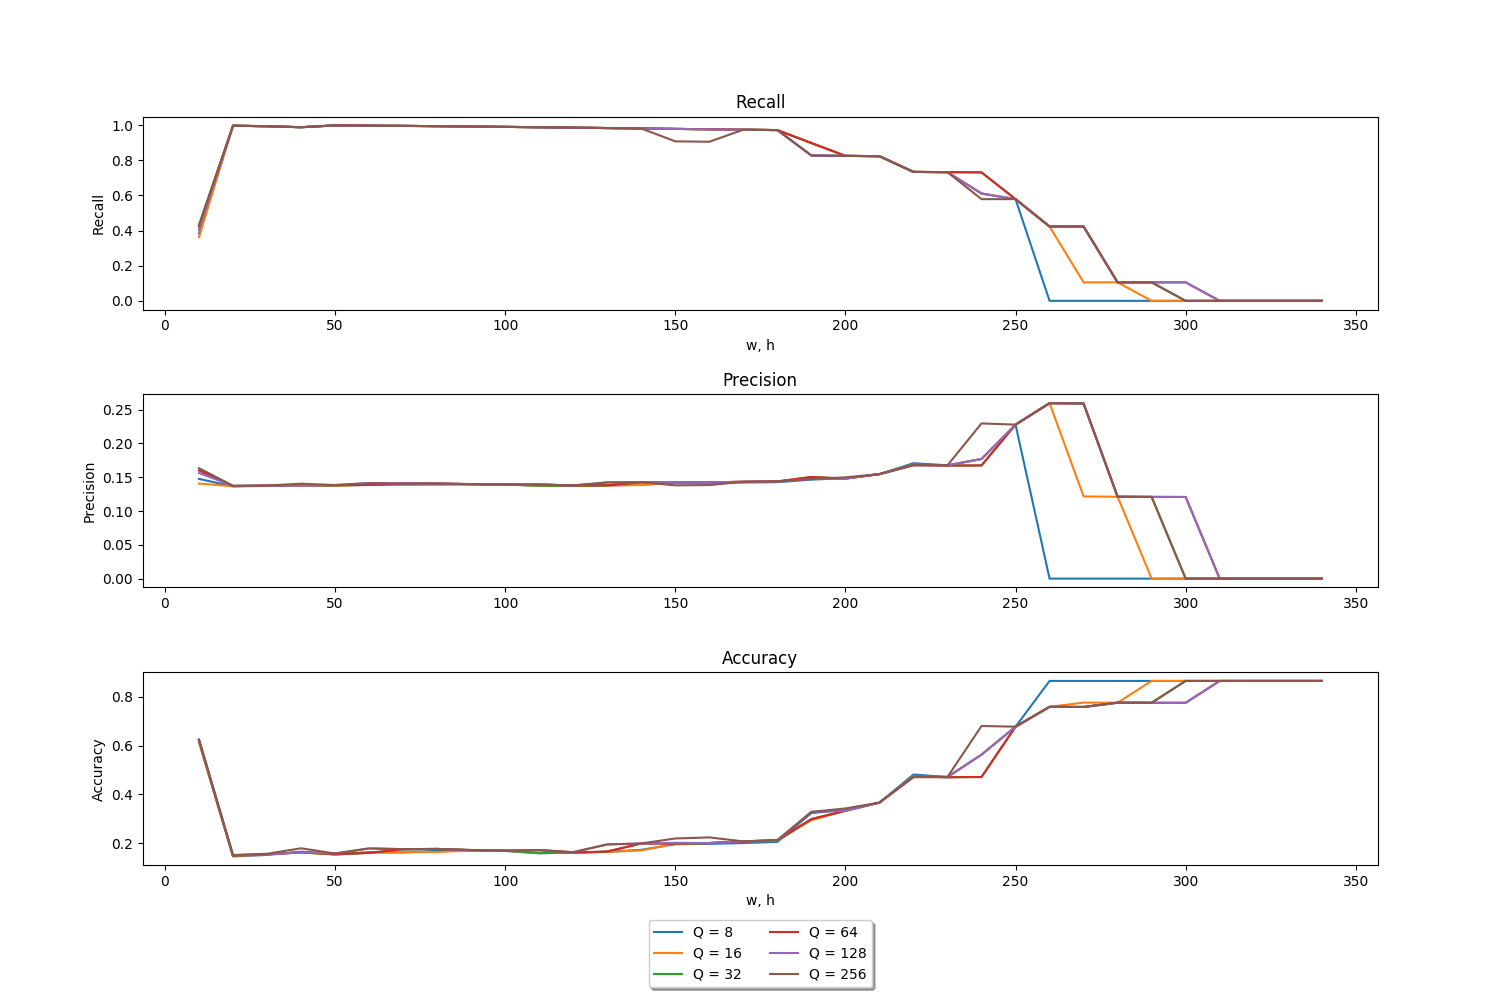
\includegraphics[width=\textwidth]{images/compare_quantification}
  \caption{Quantification}
  \label{fig:quant}
\end{figure}

\begin{figure}[H]
\centering
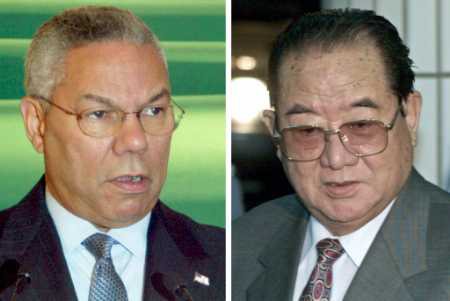
\includegraphics[width=0.3\textwidth]{images/quantified_original.png}
\caption{Image originale}
\end{figure}

\begin{figure}[H]
\centering
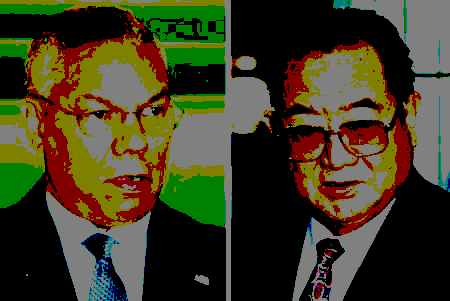
\includegraphics[width=0.3\textwidth]{images/quantified_test2.png}\hfill
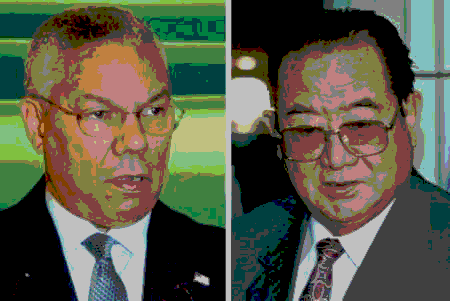
\includegraphics[width=0.3\textwidth]{images/quantified_test4.png}\hfill
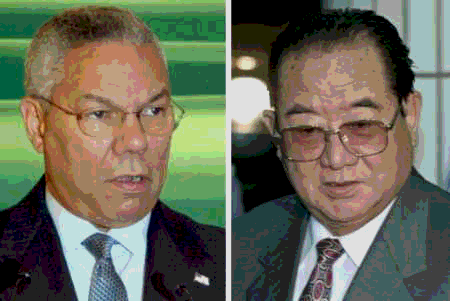
\includegraphics[width=0.3\textwidth]{images/quantified_test8.png}\hfill
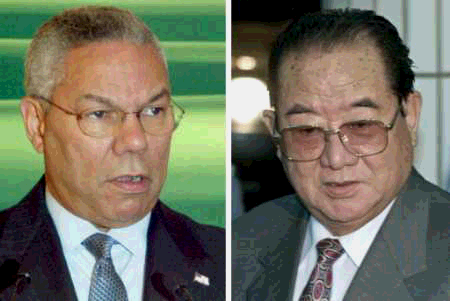
\includegraphics[width=0.3\textwidth]{images/quantified_test16.png}\hfill
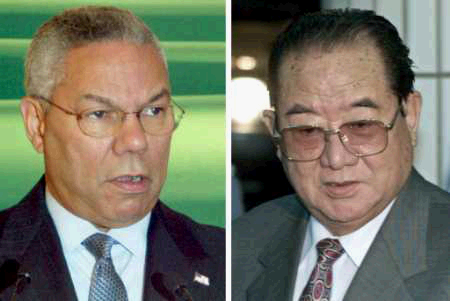
\includegraphics[width=0.3\textwidth]{images/quantified_test32.png}\hfill
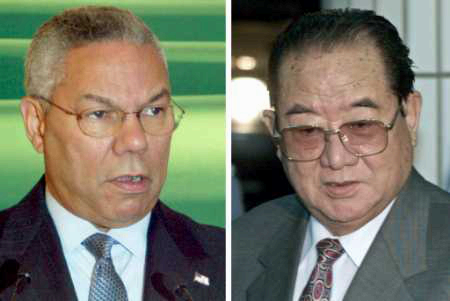
\includegraphics[width=0.3\textwidth]{images/quantified_test64.png}\hfill
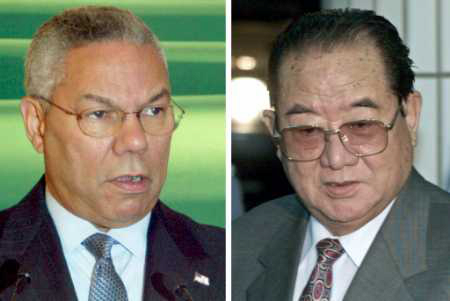
\includegraphics[width=0.3\textwidth]{images/quantified_test128.png}
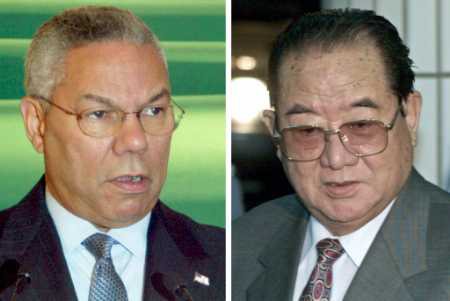
\includegraphics[width=0.3\textwidth]{images/quantified_test256.png}

\caption{Images quantifiées. De gauche à droite, de haut en bas, chaque couleur est stockée sur 1, 2, 3... jusqu'à 8 bits}
\label{fig:quantif}
\end{figure}

On constate que la quantification Q n'impacte que peu les performances pour les ellipses de taille inférieure à 150. De plus la quantification permettant un couple (recall, accuracy) le plus élevé, se situe pour des ellipses de taille d'environ 30 de hauteur et largueur.
On retrouve ce résultat grâce à la quantification des images ci-dessus, on remarque qu'à partir de Q=3, il est quasiement impossible de distinguer l'image quantifiée de l'image originale. Il y a donc assez d'information pour notre détecteur de visage.


\begin{figure}[H]
  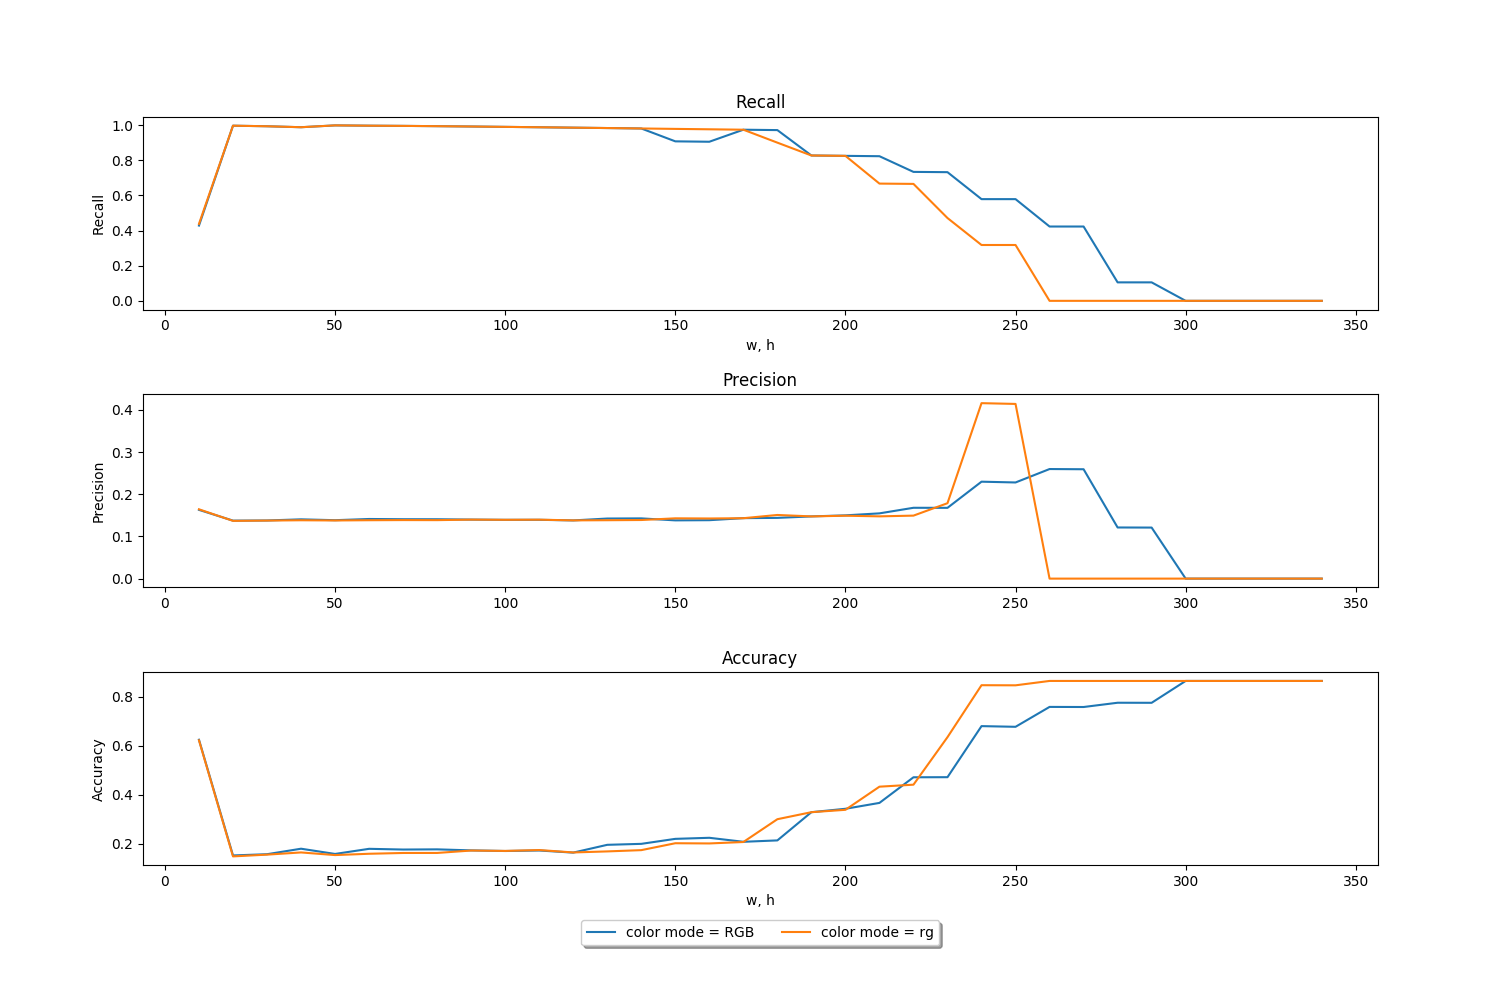
\includegraphics[width=\textwidth]{images/compare_color_mode}
  \caption{Quantification}
  \label{fig:colmode}
\end{figure}

On constate que le mode de couleur à une influence que limité sur des petites ellipseson c'est encore avec des peties ellipses que le couple(recall, accuracy) semble le meilleur.

\begin{figure}[H]
  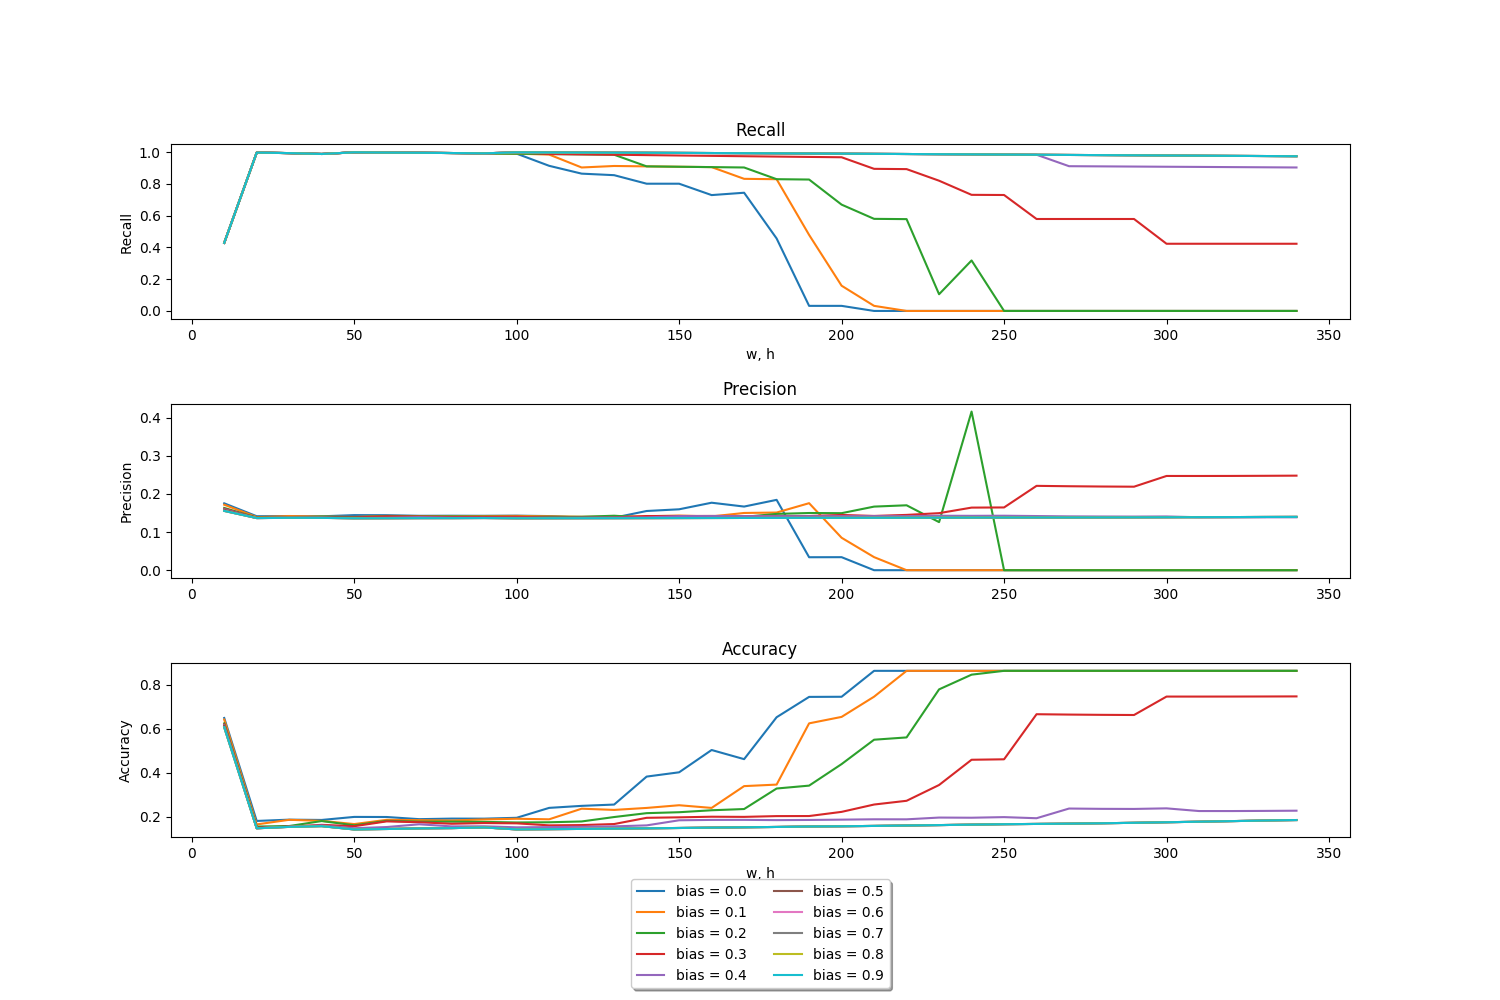
\includegraphics[width=\textwidth]{images/compare_bias}
  \caption{Biais}
  \label{fig:biais}
\end{figure}

Finalement le dernière paramètre de cette étape et le biais. Or on constate qu'il a beaucoup d'impact pour les ellipses non petite. De plus on constant qu'avec des biais élevé, le recall est presque tjs a 1 car il n'y a pas de faux négatif... De plus un bon couple RA semble aussi obtenu avec des ellises petites et un biais de $0.2$.

\subsection{Paramètres du challenge 2}
Nous allons ensuite faire varier le nombre d'angle:

\begin{figure}[H]
  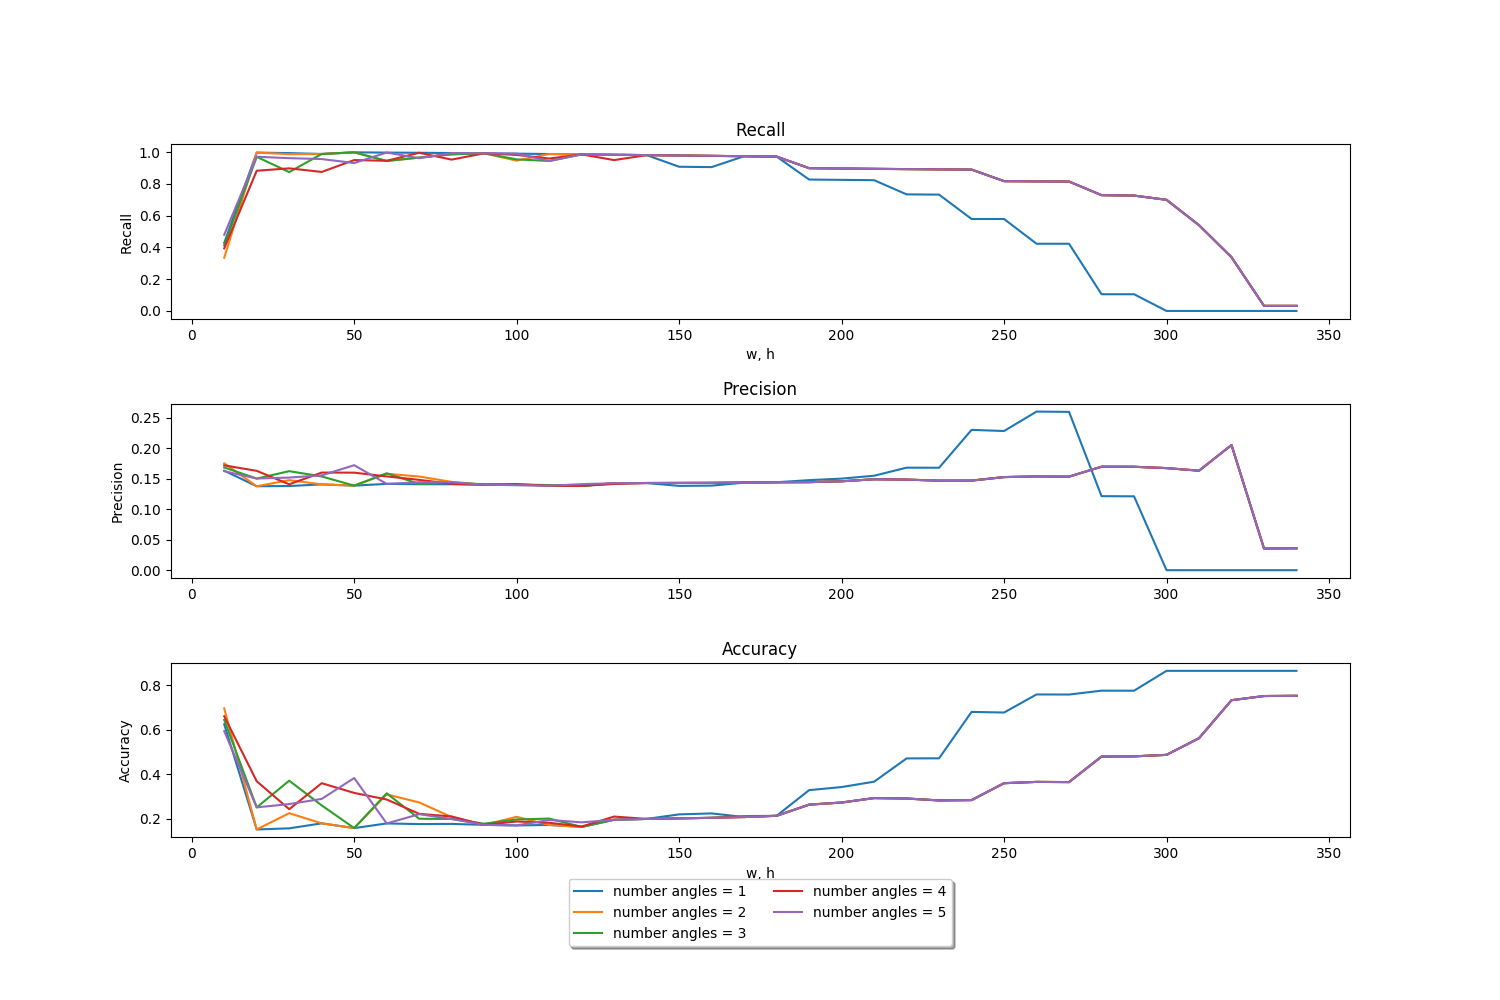
\includegraphics[width=\textwidth]{images/compare_angle}
  \caption{Nombre d'angles}
  \label{fig:angles}
\end{figure}


\subsection{Paramètres du challenge 3}

\begin{figure}[H]
  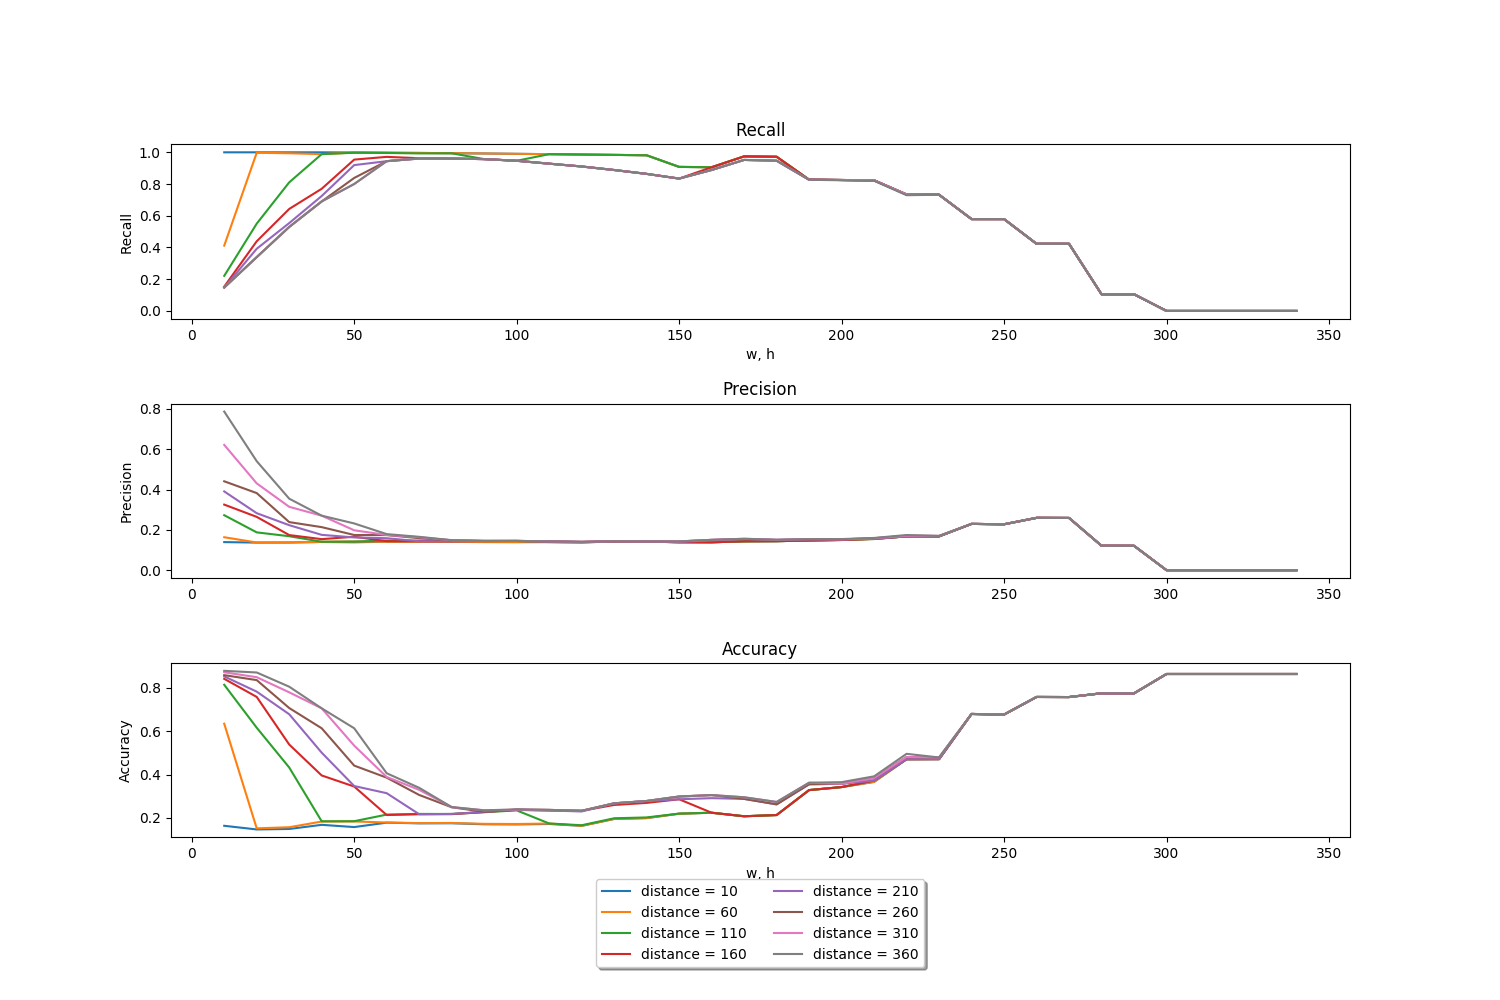
\includegraphics[width=\textwidth]{images/compare_distance}
  \caption{Nombre d'angles}
  \label{fig:dist}
\end{figure}

\subsection{Conclusion sur le choix des paramètres}
On constate que pour tous les paramètres, notre algorithme fonctionne mieux avec soit avec des ellipses petites(entre 0 et 50 de hauteur et largeur), ou avec des ellipses grande. Cependant Nous avons fait le choix de prendre des ellipses plus petites car cela permet d'avoir un bon recall et une bonne accuracy. De plus, nous avons mis en place une méthode permettant d'augmenter la précision et de maintenir c'est paramètres(cf dernière parti).

Il est à présent temps de choisir les paramètres liés à l'étape 1: Pour se faire nous avons fixer:

\begin{itemize}
  \item $Q = 256$
  \item le mode de couleur en RGB
  \item le biais: $B = 0.2$
\end{itemize}

Pour le challenge 2 et 3:

\begin{itemize}
  \item REMPLIR LES PARAMETRES PUTAIN
\end{itemize}

\#TODO : placer la ROC avec ces paramètres la wallaj

\section{Initiative : utiliser une enveloppe convexe}
D'après les analyses précédantes, nous avons remarqué qu'en utilisant de petites ellipses, on obtenait de meilleurs résultats d'un point de vu métriques. Cependant, avec ces paramètres un visage et caractérisé par plusieurs ellipses... Pour réssoudre ce problème, nous avons mis en place une enveloppe convexe qui englobe toutes les ellipses détectées dans les deux premiers challenges.
Pour tracer cette envoloppe nous avons utilisé deux algorithmes:

\begin{itemize}
  \item Un algorithme de clustering pour patitionner l'espace
  \item Un algorithme d'envoloppe convexe elliptique
\end{itemize}

\subsection{Density-Based Spatial clustering of Application with noise}
La première problème a ressoudre pour tracer l'envoloppe elliptique est de définir les groupes d'ellipses correspondant à un même visage. Pour cela nous avons utilisé un algorithme de clustering permettant de partitionner l'espace: Le DNSCAN. En effet cette algorithme permet de regrouper des points dans l'espace en plusieurs sous ensemble(cluster) de point dont le distance euclidienne ne dépasse pas une certain valeur. Ainsi nous avons appliqué cet algorithme en centre des différentes ellipses détectés par notre algorithmede reconnaissance de forme.
De plus grâce à cet algorithme, nous avons pu effacé les detections non significatives(Contre par exemple une seule ellipse...)
Nous avons fait le choix de ne pas ré-implémenter cet algorithme car il est disponible en opensource dans la library python \texttt{sklearn.cluster}.

\subsection{Ellipse convexe}
 Une fois les groupes d'ellipses correspondant à un visage isolé, nous avons fait le choix de tracer une ellipse enveloppant toutes les ellipses detectés. Pour ce faire on a utilisé la fonction fitEllipse de openCV. En effet cet fonction permet de tracer sur une image une ellipse comprennant plusieurs points. Ainsi nous avons appliqué cette fonction aux groupes de points détectés par l'algorithme DBSCAN.

 \begin{figure}[H]
   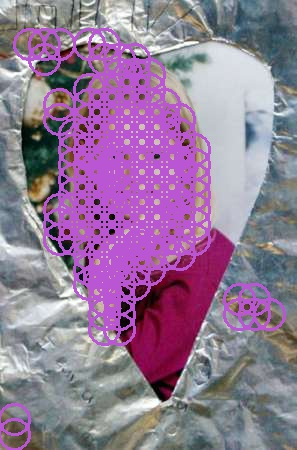
\includegraphics[width=0.5\textwidth]{images/raw_face_img_971}\hfill
   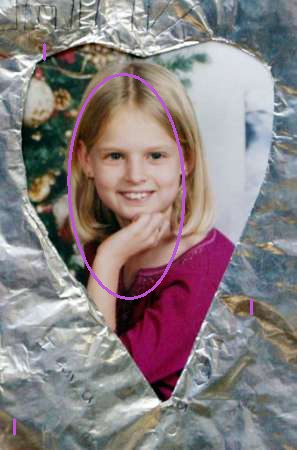
\includegraphics[width=0.5\textwidth]{images/face_img_971}\hfill
   \caption{Ellipses détectées (gauche) Ellipse finale (droite)}
   \label{fig:faces}
 \end{figure}

\subsection{Impact sur les performances}
D'un point de vue performance, cette méthode permet de gagner en précision tout en maintenant les autres paramètres. Pour tracer des courbes, on a appliquer la méthodes précédante sur les petites valeurs de h et w (w, h < 75). et on obtiens les courbes suivantes:

\begin{figure}[H]
  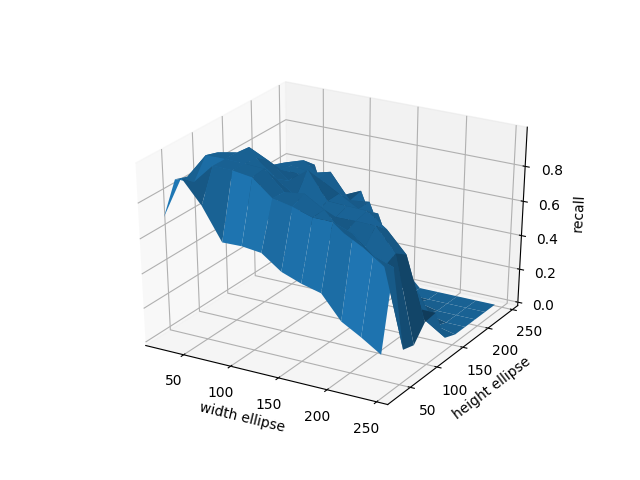
\includegraphics[width=\textwidth]{images/recall_ellipse}\hfill
  %\caption{Ellipses détectées (gauche) Ellipse finale (droite)}
  \label{fig:rec_ellipse}
\end{figure}

On observe bien que le recall ne varie presque pas pour des ellipses petites.

\begin{figure}[H]
  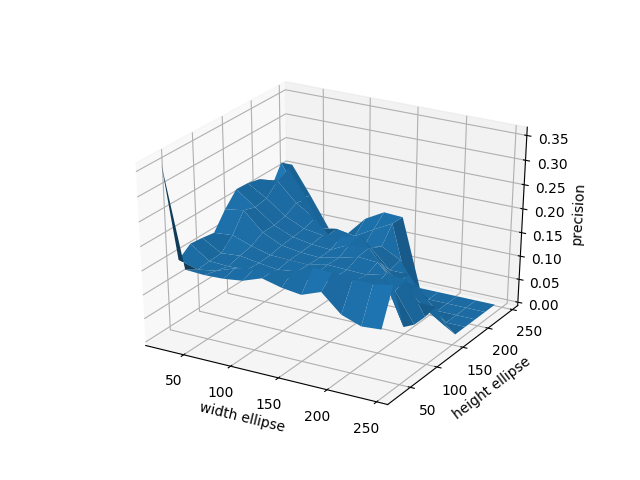
\includegraphics[width=\textwidth]{images/precision_ellipse}\hfill
  %\caption{Ellipses détectées (gauche) Ellipse finale (droite)}
  \label{fig:prec_ellipse}
\end{figure}

Cependant on observe que la precision en est presque doublée(ici mesurée sur des paramètres arbitraire d'ou la valeur faible...)

On a donc bien une méthode améliorant la performance de notre algorithme.

\section{Conclusions}

A la fin de ce premier algorithme de détection d'image, nous avons réussir à créer un algorithme qui détecte les images avec de bonnes performance. De plus nous avons mis en place une amélioration grace a des contours convexes et des algorithmes de partition de l'espace. Cependant, notre algorithme n'arrive pas à faire la différence entre les différentes parties de peau pouvant ètre présent sur une photo.

Voici le résultat de notre algorithme sur nos propres portraits.

\begin{figure}[H]
  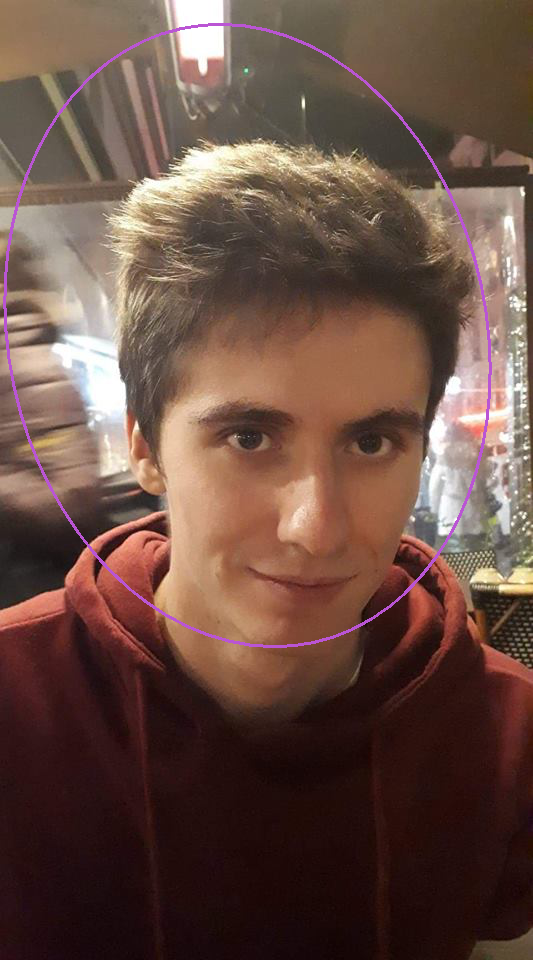
\includegraphics[width=0.3\textwidth]{images/florent20}\hfill
  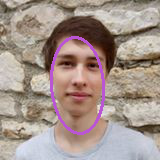
\includegraphics[width=0.3\textwidth]{images/antonin20}\hfill
  \includegraphics[width=0.3\textwidth]{images/yoan20}\hfill
  \caption{(de gauche à droite) Résultat de l'algorithme sur Florent, Antonin et Yoan}
  \label{fig:nous}
\end{figure}

%
% \appendix
%
% \bibliographystyle{authoryear-fr}
% \bibliography{references}

%%%%%%%%%%%%%%%%
%%% Abstract %%%
%%%%%%%%%%%%%%%%

% \thispagestyle{empty}
%
% \vspace*{\fill}
% \noindent\rule[2pt]{\textwidth}{0.5pt}\\
% {\textbf{Résumé ---}}
% {\textbf{Mots clés :}}
% Lorem ipsum dolor sit amet, consectetur adipiscing elit. Sed non risus. Suspendisse lectus tortor.
% \\
% \noindent\rule[2pt]{\textwidth}{0.5pt}
% \begin{center}
%   ISAE\\
%   10, avenue Édouard Belin\\
%   BP 54032\\
%   31055 Toulouse CEDEX 4
% \end{center}
% \vspace*{\fill}

\end{document}
